\documentclass{article}
\usepackage{tikz}
\usepackage{framed}
\usepackage{amsfonts}
\usepackage{amsmath}
\usepackage[bottom=1in]{geometry} 



\renewcommand\thesection{\arabic{section}}
\renewcommand\thesubsection{\arabic{subsection}}

 
\newtheorem{theorem}{Theorem}[section]
\title{An Algebraic Study on Star Patterns.}

%An Algebraic Study on Star Patterns; Geometry of Factor Groups.
\author{Rohan Thomas}
\begin{document}
\maketitle
\section{Introduction}
Consider the problem of drawing star patterns. If you are asked to draw a 5 pointed star pattern, it is relatively straight forward. How about an 8 pointed star pattern?. It could be challenging at first. To do this, start by drawing a circle and then mark equally spaced 8 points and label them 0, 1, 2, 3, $\cdots$ , 7.  Next, connect each point to another point which is at a fixed units away. For instance, let us decide to connect every point to points which are 3 units away. This means we can we connect 0 to 3, 3 to 6,$\cdots$,5 to 0 to obtain Fig 1.1. \\[2mm]
On the other hand, if the choice is to connect every point to points that are 2 units away, this choice forms a star pattern having two distinct components. To draw this pattern, we can connect 0 to 2, 2 to 4,..., 6 to 0 for the first component, and then connect 1 to 3, 3 to 5, ..., 7 to 1 to obtain Fig 1.2. Notice that the choice of turning by 3 results in construction without lifting pen; such a pattern is called as a \textit{star polygon}. In contrast, when connecting 2 units away requires lifting the pen, and this pattern is referred to as a \textit{star figure}. This means, star patterns are generally classified into star polygons and star figures.\\[2mm]
These patterns are commonly denoted using Schläfli symbol \{$n$/$k$\}, where $n$ is the number of vertices and $k$ is turning number. The star polygon obtained from connecting every third is denoted as $\{8/3\}$, while the star figure drawn by connecting every two units apart is denoted as $\{8/2\}$.

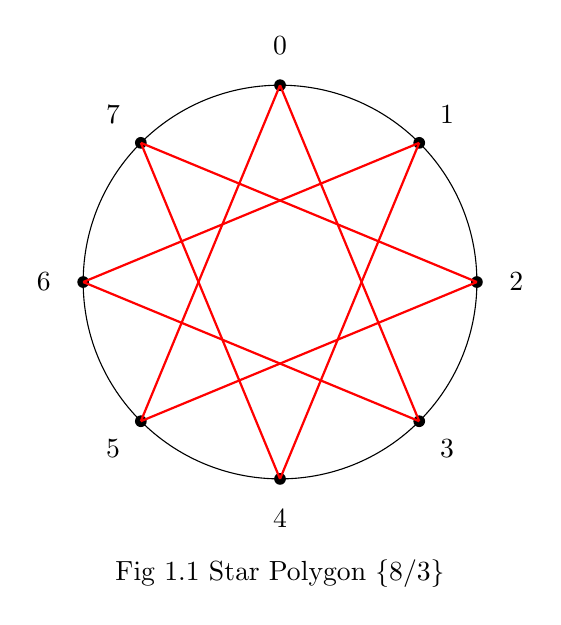
\begin{tikzpicture}
	
	\def\circRadius{2.5cm} % Radius of the circle
	\def\m{8} % Number of points
	\def\startLabel{0} % Starting label
	
	% Draw the circle
	\draw (0, 0) circle (\circRadius);
	
	% Calculate the angle between consecutive points
	\pgfmathsetmacro{\angle}{360 / \m}
	
	% Place the points and label them in clockwise order
	\foreach \i in {0, 1, ..., \numexpr\m-1} {
		\pgfmathsetmacro{\pointAngle}{90 - \i * \angle}
		\node[circle, fill, inner sep=1.5pt] at (\pointAngle:\circRadius) {};
	}
	
	% Place labels outside the circle
	\foreach \i in {0, 1, ..., \numexpr\m-1} {
		\node at (90 - \i * \angle:\circRadius + 0.5cm) {\i};
	}
	
	\draw[red, thick] (90 - 0 * \angle:\circRadius) -- (90 - 3* \angle:\circRadius);
	\draw[red, thick] (90 - 3 * \angle:\circRadius) -- (90 - 6* \angle:\circRadius);
	\draw[red, thick] (90 - 6 * \angle:\circRadius) -- (90 - 1* \angle:\circRadius);
	\draw[red, thick] (90 -1 * \angle:\circRadius) -- (90 - 4* \angle:\circRadius);
	\draw[red, thick] (90 -4 * \angle:\circRadius) -- (90 - 7* \angle:\circRadius);
	\draw[red, thick] (90 -7 * \angle:\circRadius) -- (90 - 2* \angle:\circRadius);
	\draw[red, thick] (90 -2 * \angle:\circRadius) -- (90 - 5* \angle:\circRadius);
	\draw[red, thick] (90 -5 * \angle:\circRadius) -- (90 - 0* \angle:\circRadius);
	
	\node[below] at (0,-3.4) {Fig 1.1 Star Polygon \{8/3\}};    
	
	\hspace{8cm}
	\def\circRadius{2.5cm} % Radius of the circle
	\def\m{8} % Number of points
	\def\startLabel{0} % Starting label
	
	% Draw the circle
	\draw (0, 0) circle (\circRadius);
	
	% Calculate the angle between consecutive points
	\pgfmathsetmacro{\angle}{360 / \m}
	
	% Place the points and label them in clockwise order
	\foreach \i in {0, 1, ..., \numexpr\m-1} {
		\pgfmathsetmacro{\pointAngle}{90 - \i * \angle}
		\node[circle, fill, inner sep=1.5pt] at (\pointAngle:\circRadius) {};
	}
	
	% Place labels outside the circle
	\foreach \i in {0, 1, ..., \numexpr\m-1} {
		\node at (90 - \i * \angle:\circRadius + 0.5cm) {\i};
	}
	
	\draw[red, thick] (90 - 0 * \angle:\circRadius) -- (90 - 2* \angle:\circRadius);
	\draw[red, thick] (90 - 1 * \angle:\circRadius) -- (90 - 3* \angle:\circRadius);
	\draw[red, thick] (90 - 3* \angle:\circRadius) -- (90 - 5* \angle:\circRadius);
	\draw[red, thick] (90 - 5* \angle:\circRadius) -- (90 - 7* \angle:\circRadius);
	\draw[red, thick] (90 - 7* \angle:\circRadius) -- (90 - 9* \angle:\circRadius);
	\draw[red, thick] (90 - 2 * \angle:\circRadius) -- (90 - 4* \angle:\circRadius);
	\draw[red, thick] (90 - 4 * \angle:\circRadius) -- (90 - 6* \angle:\circRadius);
	\draw[red, thick] (90 - 6 * \angle:\circRadius) -- (90 - 0* \angle:\circRadius);
	
	
	\node[below] at (0,-3.4) {Fig 1.2 Star Figure \{8/2\}}; 
\end{tikzpicture}
\\[2mm]
It's a fun activity to observe and make conjectures about these patterns. For instance, How many $n$ pointed star polygons can be drawn , or How many distinct components are there in a star figure. We will discuss the algebraic connections in star polygons and figures to answer these questions. In fact, these patterns will help us to visualize abstract concepts from Group theory such as cyclic groups, isomorphism and cosets. Let us begin by considering the construction and discussion of star patterns without lifting the pen or better known as star polygons.
\section{Star Polygons: Construction and Their Cyclic Structure}

As suggested in the introduction, when constructing a star polygon, we need to choose the turning number such that it doesn't loop in a smaller subset of the labels but reach all them. This is exactly the situation when we choose $k$ such that $\gcd(k,n) =1$ 
\begin{framed}
	Draw a circle and mark $n$ points and label them with numbers from 0 to $m-1$. Choose any number $k$ such that $\gcd(k,n)=1$. Join each point $x$ to $(x+k)$ $\pmod{n}$.
\end{framed}

For instance, The following are possible 7 pointed star polygons based on this procedure:
\begin{center}
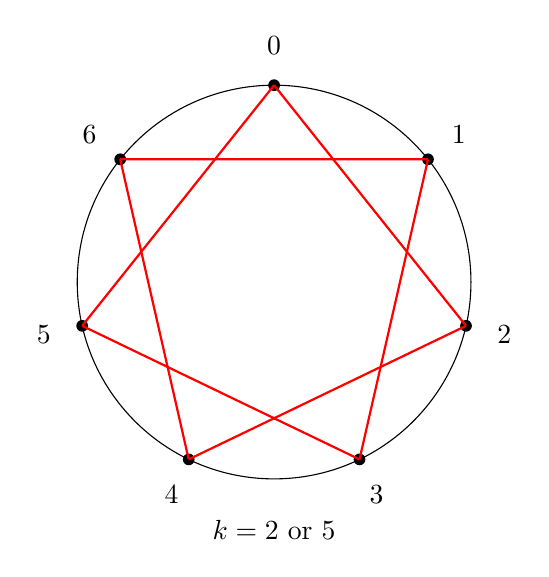
\begin{tikzpicture}
		\def\circRadius{2.5cm} % Radius of the circle
		\def\m{7} % Number of points
		\def\startLabel{0} % Starting label
		
		% Draw the circle
		\draw (0, 0) circle (\circRadius);
		
		% Calculate the angle between consecutive points
		\pgfmathsetmacro{\angle}{360 / \m}
		
		% Place the points and label them in clockwise order
		\foreach \i in {0, 1, ..., \numexpr\m-1} {
			\pgfmathsetmacro{\pointAngle}{90 - \i * \angle}
			\node[circle, fill, inner sep=1.5pt] at (\pointAngle:\circRadius) {};
		}
		
		% Place labels outside the circle
		\foreach \i in {0, 1, ..., \numexpr\m-1} {
			\node at (90 - \i * \angle:\circRadius + 0.5cm) {\i};
		}
		\draw[red, thick] (90 - 0 * \angle:\circRadius) -- (90 - 2 * \angle:\circRadius);
		\draw[red, thick] (90 - 2 * \angle:\circRadius) -- (90 - 4 * \angle:\circRadius);
		\draw[red, thick] (90 - 4 * \angle:\circRadius) -- (90 - 6 * \angle:\circRadius);
		\draw[red, thick] (90 - 6 * \angle:\circRadius) -- (90 - 8 * \angle:\circRadius);
		\draw[red, thick] (90 - 8 * \angle:\circRadius) -- (90 - 10 * \angle:\circRadius);
		\draw[red, thick] (90 - 10 * \angle:\circRadius) -- (90 - 12 * \angle:\circRadius);
		\draw[red, thick] (90 - 12 * \angle:\circRadius) -- (90 - 14 * \angle:\circRadius);
		\node[below] at (0,-2.9) {$k=2$ or 5};
	\end{tikzpicture}    
	\hspace{1cm}
	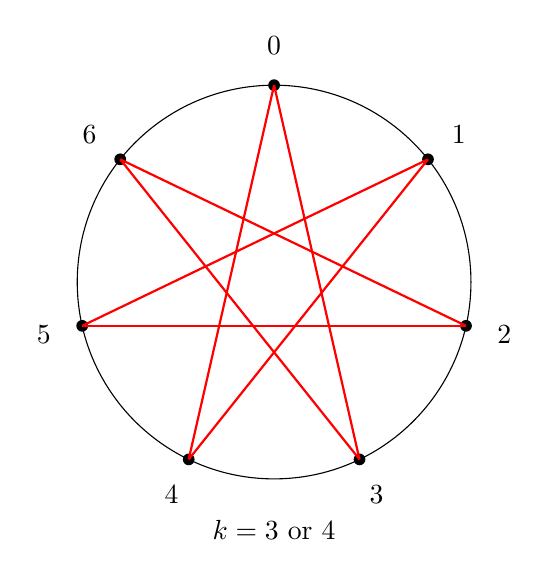
\begin{tikzpicture}
		\def\circRadius{2.5cm} % Radius of the circle
		\def\m{7} % Number of points
		\def\startLabel{0} % Starting label
		
		% Draw the circle
		\draw (0, 0) circle (\circRadius);
		
		% Calculate the angle between consecutive points
		\pgfmathsetmacro{\angle}{360 / \m}
		
		% Place the points and label them in clockwise order
		\foreach \i in {0, 1, ..., \numexpr\m-1} {
			\pgfmathsetmacro{\pointAngle}{90 - \i * \angle}
			\node[circle, fill, inner sep=1.5pt] at (\pointAngle:\circRadius) {};
		}
		
		% Place labels outside the circle
		\foreach \i in {0, 1, ..., \numexpr\m-1} {
			\node at (90 - \i * \angle:\circRadius + 0.5cm) {\i};
		}
		\draw[red, thick] (90 - 0 * \angle:\circRadius) -- (90 - 3 * \angle:\circRadius);
		\draw[red, thick] (90 - 3 * \angle:\circRadius) -- (90 - 6 * \angle:\circRadius);
		\draw[red, thick] (90 - 6 * \angle:\circRadius) -- (90 - 2 * \angle:\circRadius);
		\draw[red, thick] (90 - 2 * \angle:\circRadius) -- (90 - 5 * \angle:\circRadius);
		\draw[red, thick] (90 - 5 * \angle:\circRadius) -- (90 - 1 * \angle:\circRadius);
		\draw[red, thick] (90 - 1 * \angle:\circRadius) -- (90 - 4 * \angle:\circRadius);
		\draw[red, thick] (90 - 4 * \angle:\circRadius) -- (90 - 0 * \angle:\circRadius);
		\node[below] at (0,-2.9) {$k=3$ or 4};    
	\end{tikzpicture}    
	\hspace{1cm}
	
	\end{center}
	
	\begin{center}
	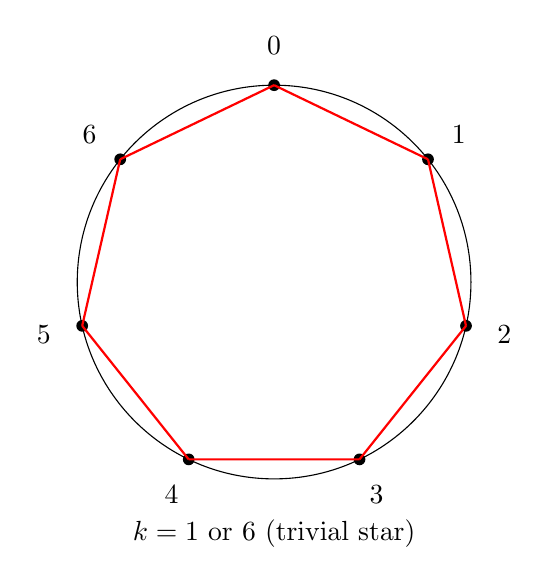
\begin{tikzpicture}
		\def\circRadius{2.5cm} % Radius of the circle
		\def\m{7} % Number of points
		\def\startLabel{0} % Starting label
		
		% Draw the circle
		\draw (0, 0) circle (\circRadius);
		
		% Calculate the angle between consecutive points
		\pgfmathsetmacro{\angle}{360 / \m}
		
		% Place the points and label them in clockwise order
		\foreach \i in {0, 1, ..., \numexpr\m-1} {
			\pgfmathsetmacro{\pointAngle}{90 - \i * \angle}
			\node[circle, fill, inner sep=1.5pt] at (\pointAngle:\circRadius) {};
		}
		
		% Place labels outside the circle
		\foreach \i in {0, 1, ..., \numexpr\m-1} {
			\node at (90 - \i * \angle:\circRadius + 0.5cm) {\i};
		}
		\draw[red, thick] (90 - 0 * \angle:\circRadius) -- (90 - 1 * \angle:\circRadius);
		\draw[red, thick] (90 - 1 * \angle:\circRadius) -- (90 - 2 * \angle:\circRadius);
		\draw[red, thick] (90 - 2 * \angle:\circRadius) -- (90 - 3 * \angle:\circRadius);
		\draw[red, thick] (90 - 3 * \angle:\circRadius) -- (90 - 4 * \angle:\circRadius);
		\draw[red, thick] (90 - 4 * \angle:\circRadius) -- (90 - 5 * \angle:\circRadius);
		\draw[red, thick] (90 - 5 * \angle:\circRadius) -- (90 - 6 * \angle:\circRadius);
		\draw[red, thick] (90 - 6 * \angle:\circRadius) -- (90 - 0 * \angle:\circRadius);
		\node[below] at (0,-2.9) {$k=1$ or 6 (trivial star)};
	\end{tikzpicture}
\end{center}
\newpage
In this section, we will mainly address following questions:

\begin{itemize}
	\item Why the condition $\gcd(k,n) = 1$?
	\item How many $n$ pointed star polygons can be drawn. ?
	\item Why do star polygon symmetries pair up ?
\end{itemize}
In addition to answer these questions, we need to understand cyclic groups, the underlying algebra structure associated with these patterns. In fact they help to visualize cyclic groups. Let us first introduce the notion of a cyclic group.

\subsection*{Cyclic Groups; An overview}
Given a set $G$ together with an binary operation $*$, we say G forms an algebraic structure named \textit{group}, if it satisfies the following axioms,
\begin{enumerate}
    \item $*$ is a binary operation in G
    \item $a*(b*c)=(a*b)*c$, $\forall a,b,c \in G$
    \item there exist $e \in G$ such that $a*e=e*a=a$
    \item for each $a \in G$ there exist b such that $a*b=e=b*a$
\end{enumerate}
A group G is \underline{said to be \textit{cyclic}}, if there exist $a \in G$ such that $G=\{a^{n}:n \in \mathbb{Z}\}$, where $'a'$ is called as the generator. In other words, a cyclic group posses an element that can generate all other elements in the group. An important example of cyclic group is an additive group. Let $\mathbb{Z}_n =\{0,1,2,3,\ldots,(n-1)\}$ be the set of remainders upon division by $n$, we can easily verify $\mathbb{Z}_n$ is a group under addition modulo $n$. Since 1 $\in$  $\mathbb{Z}_n$, clearly it is cyclic.\\[2mm]
The construction procedure suggested earlier be thought as constructing over the cyclic group $\mathbb{Z}_n$. We can think of wrapping around elements of $\mathbb{Z}_n$ around the circle, , choosing an element $k$ from $\mathbb{Z}_n$ and connecting the points by computing $k, (k +_n k) , (k +_n k +_n k),\cdots, 0$.

\subsection*{Why the condition $\gcd(k,n)=1$?}
As our intuition suggests, an $n$ pointed star polygons is only possible when the choice of $k$ is a generator of the group $\mathbb{Z}_ n$. If you observe Fig 2.1, we can note that when $m$ = 8 and $k = 2$, this choice reaches all the multiples of 2. Similarly, $k = 6$ reaches the same labels. What's common between them ? They share the greatest common divisor of 2 with $m =8$. In fact, when we choose some $k$, the labels it will reach are multiples $\gcd(k,n)$. So naturally to reach all the labels $\gcd(k,n)$ simply has to be 1. The following theorem proves it formally using bezout's identity and congruence properties. 

\begin{theorem}
	$k \in \mathbb{Z}_n$ is a generator of $\mathbb{Z}_n,$ if $\gcd(k,n)=1$
\end{theorem}
\textbf{Proof}: The idea of proof is similar to earlier discussion. We have to show that, if $gcd(k,n)=1$, then the successive elements $k, (k +_n k) , (k +_n k +_n k),$ somehow reaches 1. If it can reach 1 then it must reach any arbitrary $b \in \mathbb{Z}_n$.\\[2mm]
Applying bezout's identity in $\gcd(a,n)=1$, we get $x_0, y_0$ such that $ax_0 +ny_0=1$. Rearranging we get, $ax_0-1=n(-y_0)$. From the definition of congruence, this will imply $ax_0 \equiv 1 \pmod{n}$. Now let $b \in \mathbb{Z}_n$ be arbitrary , using the multiplication property of congruence we get
$$a(x_0b) \equiv (b) \pmod{n}\implies \underbrace{a +_n a +_n \ldots +_n a}_{x_0b \text{ times}} = b$$
\\

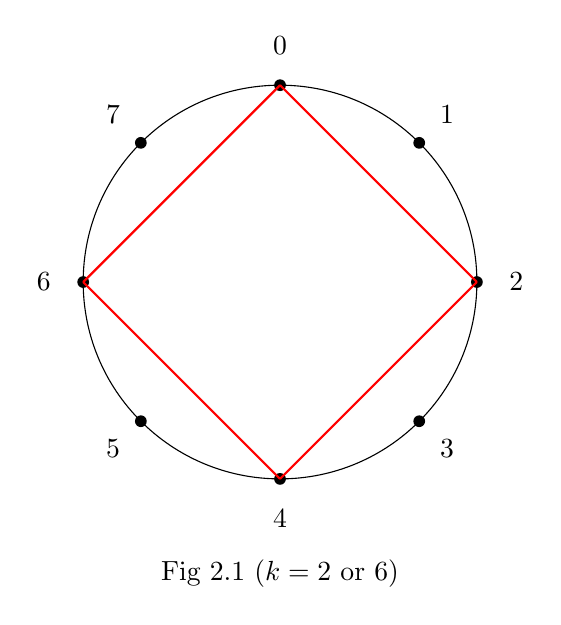
\begin{tikzpicture}
	\def\circRadius{2.5cm} % Radius of the circle
	\def\m{8} % Number of points
	\def\startLabel{0} % Starting label
	
	% Draw the circle
	\draw (0, 0) circle (\circRadius);
	
	% Calculate the angle between consecutive points
	\pgfmathsetmacro{\angle}{360 / \m}
	
	% Place the points and label them in clockwise order
	\foreach \i in {0, 1, ..., \numexpr\m-1} {
		\pgfmathsetmacro{\pointAngle}{90 - \i * \angle}
		\node[circle, fill, inner sep=1.5pt] at (\pointAngle:\circRadius) {};
	}
	
	% Place labels outside the circle
	\foreach \i in {0, 1, ..., \numexpr\m-1} {
		\node at (90 - \i * \angle:\circRadius + 0.5cm) {\i};
	}
	
	\draw[red, thick] (90 - 0 * \angle:\circRadius) -- (90 - 2* \angle:\circRadius);
	\draw[red, thick] (90 - 2 * \angle:\circRadius) -- (90 - 4* \angle:\circRadius);
	\draw[red, thick] (90 - 4 * \angle:\circRadius) -- (90 - 6* \angle:\circRadius);
	\draw[red, thick] (90 - 6 * \angle:\circRadius) -- (90 - 0* \angle:\circRadius);
	
	
	\node[below] at (0,-3.4) {Fig 2.1 ($k = 2$ or $6$)}; 
	\hspace{8cm}
	\def\circRadius{2.5cm} % Radius of the circle
	\def\m{8} % Number of points
	\def\startLabel{0} % Starting label
	
	% Draw the circle
	\draw (0, 0) circle (\circRadius);
	
	% Calculate the angle between consecutive points
	\pgfmathsetmacro{\angle}{360 / \m}
	
	% Place the points and label them in clockwise order
	\foreach \i in {0, 1, ..., \numexpr\m-1} {
		\pgfmathsetmacro{\pointAngle}{90 - \i * \angle}
		\node[circle, fill, inner sep=1.5pt] at (\pointAngle:\circRadius) {};
	}
	
	% Place labels outside the circle
	\foreach \i in {0, 1, ..., \numexpr\m-1} {
		\node at (90 - \i * \angle:\circRadius + 0.5cm) {\i};
	}
	
	\draw[red, thick] (90 - 0 * \angle:\circRadius) -- (90 - 4* \angle:\circRadius);
	
	
	\node[below] at (0,-3.4) {Fig 2.2 ($k = 4$)};
	    
\end{tikzpicture}
\\
Though the choice of $k=2$ and $k=4$ didn't draw the star but they help to visualize subgroups of $\mathbb{Z}_ 8$. Fig 2.1 represents the cyclic subgroup generated by 2 or $<2> = \{0,2,4,6\}$ and Fig 2.2 represents $<4> =\{4,0\}$.

\subsection*{How many $n$ pointed star polygons can be drawn ?}
We expect to draw a star polygon for each $k \in \mathbb{Z}_ n$ such that $\gcd(k,n) = 1$. Therefore, counting those elements less than $n$ and relatively prime to $n$ will give us the possible choices of $k$. This is exactly same situation with Euler's Totient Function $\phi(n)$. Intuitively, we can see that each clockwise-construction is paired off with a counter-clockwise construction. Therefore, there are $\frac{\phi(n)}{2}$ distinct star polygons (counting the trivial star polygon). For instance, when $m =8$, $\phi(8) = 4$, so the two distinct star patterns; The trival star and Fig 1.1
\subsection*{Why do symmetries pair up?}
The fact that counter clock-wise constructions with $k$ is always paired off with clockwise construction with $(n-k)$ can be seen as a geometrical argument for why Euler's Totient Function is always even. Formally, if $k\in \mathbb{Z}_n$  is a generator then $(n-k)$ is also a generator of $\mathbb{Z}_n$.
\begin{theorem}
if $\gcd(k,n)=1$ then $\gcd(n-k,n)=1$
\end{theorem}
\textbf{Proof} (By contra-position): Suppose $\gcd(m-k,m)=d \neq 1$. Thus $d|(m-k)$ and $d|m$. from $d|(m-k)$ we get $(m-k)=dk$, for some $k \in \mathbb{Z}$. also from $d|m$ we get $m=dl$, for some $l \in \mathbb{Z}$\\[2mm]
We can easily replace m and see, $dl-k=dk \implies k=d(l-k)$. 
Thus $d|k$, but notice since $d>1$ this contradicts $(k,m)=1$ being greatest common divisor. Hence $(m-k,m)=1$\\[2mm]
The proof effectively tells us that $k$ and $(n-k)$ as not just additive inverse in the additive group but they both generator of the group.\\[2mm]
Finally, We are looking for the smallest possible non trivial star. Since the generators are always paired up. We need $\phi(n) = 4$, so that two choices belongs to trivial star and other two are our desired. This happens when we have $n=5$, because $\phi(5) = 4$ Therefore, the smallest possible star is our familiar 5 pointed star.\\

\newpage
\section{Multiplicative Construction and Isomorphism}
In the previous section, we considered the successive elements in an additive fashion to construct the pattern. It's natural to ask, can we construct a star polygon in a multiplicative fashion ?. This means, starting with the labels $\{1,2,3,...,n-1\}$ and choosing some label to repeatedly multiply and reach all elements of the set to draw a star. It turns out that we cannot do this all the time, but it's possible when $n$ is some prime number. The interesting fact is that this construction doesn't even look anywhere close to a star until we apply some magic over it, the isomorphism.\\[2mm]
Let us begin with $U(p)$, the of all positive integers less than $p$ and relatively prime to $p$.
$$U(p) = \{x : \gcd(x,p) =1\} = \{1,2,...,p-1\}$$
We can easily see that $U(p)$ is a group under multiplication modulo $p$. In general, $U(n)$ is not cyclic that is why we don't get star patterns all the time but when $n = p$, it's cyclic group.\\[2mm]
Consider $U(11) = \{1,2,3,...,10\}$. Labels these points around a circle. We can verify that 7 is a generator of the group. Thus, compute the multiplicative powers of 7 in modulo 11 and join the labels. Connect 1 to 7, 7 to $7^2 = 5$, 5 to $7^3 = 2$, 2 to $7^4 = 4$, $\cdots$ , and 8 to $7^{10} = 1$ to obtain the Figure 2.1 

\begin{center}
	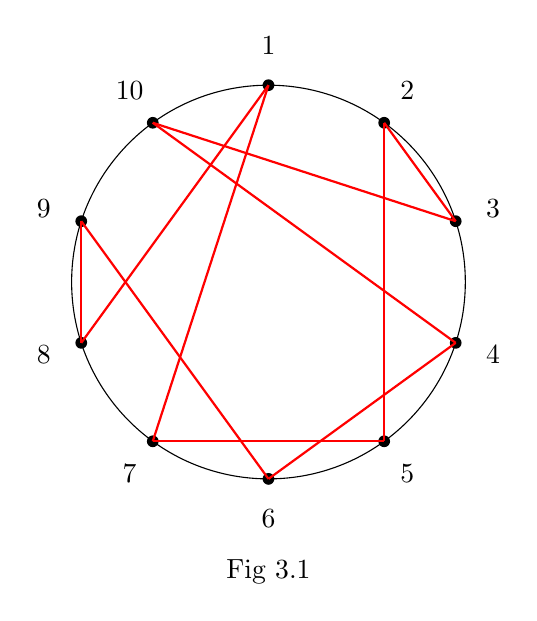
\begin{tikzpicture}
		\def\circRadius{2.5cm} % Radius of the circle
		\def\m{10} % Number of points
		
		% Draw the circle
		\draw (0, 0) circle (\circRadius);
		
		% Calculate the angle between consecutive points
		\pgfmathsetmacro{\angle}{360 / \m}
		
		% Place the points and label them in clockwise order
		\foreach \i in {0, 1, ..., \numexpr\m-1} {
			\pgfmathsetmacro{\pointAngle}{90 - \i * \angle}
			\node[circle, fill, inner sep=1.5pt] at (\pointAngle:\circRadius) {};
		}
		
		% Place labels outside the circle
		\foreach \i in {1, 2, ..., \m} {
			\pgfmathsetmacro{\labelAngle}{90 - (\i - 1) * \angle}
			\node at (\labelAngle:\circRadius + 0.5cm) {\i};
		}
		
		% Draw red lines following powers of 7 modulo 11
		\draw[red, thick] (90 - 0 * \angle:\circRadius) -- (90 - 6 * \angle:\circRadius);  % 1 -> 7
		\draw[red, thick] (90 - 6 * \angle:\circRadius) -- (90 - 4 * \angle:\circRadius);  % 7 -> 5
		\draw[red, thick] (90 - 4 * \angle:\circRadius) -- (90 - 1 * \angle:\circRadius);  % 5 -> 2
		\draw[red, thick] (90 - 1 * \angle:\circRadius) -- (90 - 2 * \angle:\circRadius);  % 2 -> 3
		\draw[red, thick] (90 - 2 * \angle:\circRadius) -- (90 - 9 * \angle:\circRadius);  % 3 -> 10
		\draw[red, thick] (90 - 9 * \angle:\circRadius) -- (90 - 3 * \angle:\circRadius);  % 10 -> 4
		\draw[red, thick] (90 - 3 * \angle:\circRadius) -- (90 - 5 * \angle:\circRadius);  % 4 -> 6
		\draw[red, thick] (90 - 5 * \angle:\circRadius) -- (90 - 8 * \angle:\circRadius);  % 6 -> 9
		\draw[red, thick] (90 - 8 * \angle:\circRadius) -- (90 - 7 * \angle:\circRadius);  % 9 -> 8
		\draw[red, thick] (90 - 7 * \angle:\circRadius) -- (90 - 0 * \angle:\circRadius);  % 8 -> 1
		
		\node[below] at (0,-3.4) {Fig 3.1};
	\end{tikzpicture}
\end{center}
Clearly it doesn't look like a star, but let's relabel these points in some fashion preserving the multiplication operation\\[2mm]
Let's observe, the following multiplication $8 = 7^{9}$ and $7 = 7^1$in $U(11)$
$$7^{9} \cdot_{11} 7^ 1 = 7^{10} = 7^{0} = 1$$\\
Notice that even though the multiplication is $U(11)$, in the exponents, an addition modulo 10 operation is happening under the hood. This means, the element $27^9$ in $U(11)$ can be corresponded to element 9 in $\mathbb{Z}_{}$. Therefore we expect a structural similarity between the groups $U(11)$ and $\mathbb{Z}_n$. This similarity can be established by an isomorphism.\\[2mm]
Let's define the isomorphism,
$$\phi(7^k\pmod{11}) = k \pmod{10}$$\\
We have the following mappings from $\mathbb{Z}_{10}$ to $U(11)$. $0 \leftrightarrow 1, 1 \leftrightarrow 2, 2 \leftrightarrow 4, 3 \leftrightarrow 8, \cdots , 9 \leftrightarrow 6.$ 
 
 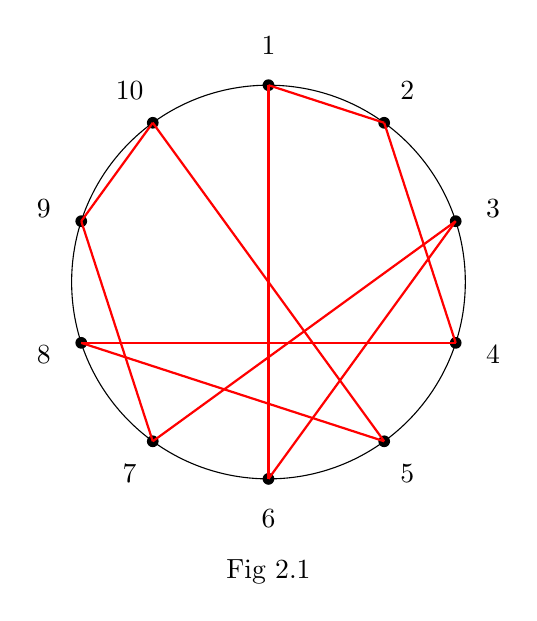
\begin{tikzpicture}
 	\def\circRadius{2.5cm} % Radius of the circle
 	\def\m{10} % Number of points
 	\def\startLabel{1} % Starting label
 	
 	% Draw the circle
 	\draw (0, 0) circle (\circRadius);
 	
 	% Calculate the angle between consecutive points
 	\pgfmathsetmacro{\angle}{360 / \m}
 	
 	% Place the points and label them in clockwise order
 	\foreach \i in {0, 1, ..., \numexpr\m-1} {
 		\pgfmathsetmacro{\pointAngle}{90 - \i * \angle}
 		\node[circle, fill, inner sep=1.5pt] at (\pointAngle:\circRadius) {};
 	}
 	
 	% Place labels outside the circle
 	\foreach \i in {1, 2, ..., \m} {
 		\pgfmathsetmacro{\labelAngle}{90 - (\i - 1) * \angle}
 		\node at (\labelAngle:\circRadius + 0.5cm) {\i};
 	}
 	
 	\draw[red, thick] (90 - 0 * \angle:\circRadius) -- (90 - 1 * \angle:\circRadius);
 	\draw[red, thick] (90 - 1 * \angle:\circRadius) -- (90 - 3 * \angle:\circRadius);
 	\draw[red, thick] (90 - 3 * \angle:\circRadius) -- (90 - 7 * \angle:\circRadius);
 	\draw[red, thick] (90 - 4 * \angle:\circRadius) -- (90 - 7 * \angle:\circRadius);
 	\draw[red, thick] (90 - 4 * \angle:\circRadius) -- (90 - 9 * \angle:\circRadius);
 	\draw[red, thick] (90 - 9 * \angle:\circRadius) -- (90 - 8 * \angle:\circRadius);
 	\draw[red, thick] (90 - 8 * \angle:\circRadius) -- (90 - 6 * \angle:\circRadius);
 	\draw[red, thick] (90 - 6 * \angle:\circRadius) -- (90 - 2 * \angle:\circRadius);
 	\draw[red, thick] (90 - 2 * \angle:\circRadius) -- (90 - 5 * \angle:\circRadius);
 	\draw[red, thick] (90 - 5 * \angle:\circRadius) -- (90 - 0 * \angle:\circRadius);
 	
 	\node[below] at (0,-3.4) {Fig 2.1};
 	
 	\hspace{4cm} $\overset{\displaystyle\varphi}{\xrightarrow{\hspace{1cm}}}$
 
 
 	
 	
 	
 \end{tikzpicture}
\end{document}

%We can think of collecting all the multiplicative inverses from $\mathbb{Z}_n$ and forming a group under multiplication. $U(n)$ doesn't always have an element called the primitive root which can generate all other elements. For example, $U(6)$ is not cyclic. Therefore we don't expect to draw star patterns all the time
%
%U(n)$ is not cyclic for any $n$, for example $U(6)$. Therefore, we don't expect to see star patterns all the time. It turns out that when $n = p$, where $p$ is some prime number. $U(p)$ is a cyclic group, or  This statement is better known as the Primitive Root Theorem\\[2mm]
%onsider $U(11) = \{1,2,3,4,...,10\}$, choose $k =2$ %